\section{最大模原理}

参见 Rudin《实分析与复分析》.

This chaper contains further generealizations of the maximum modulus theorem, as well as some rather striking applications of it, and it concludes with a theorem which shows that the maximum property "almost" characterizes the class of holomorphic functions.

\begin{figure}[H]
\centering
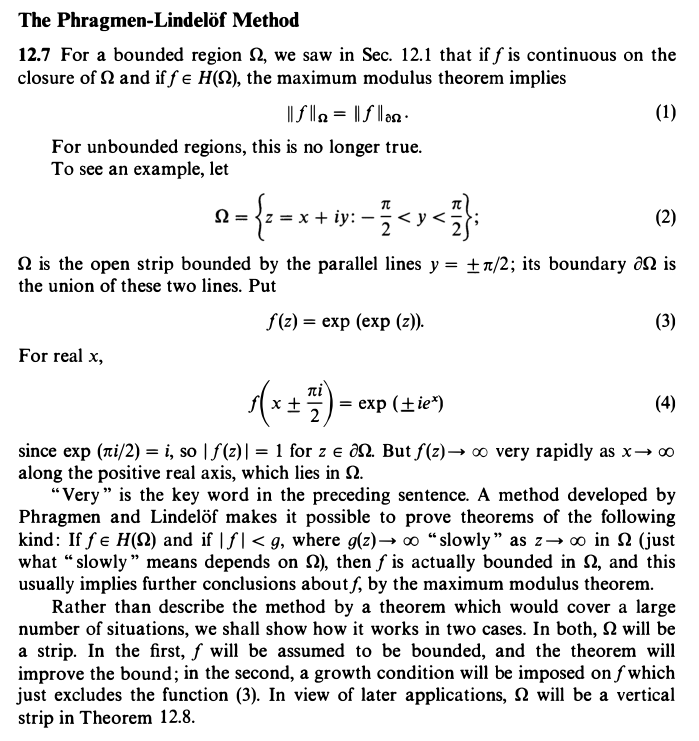
\includegraphics[width=\textwidth]{最大模原理-2025040417.png}
% \caption{}
\label{}
\end{figure}

\subsection{An example concerning the increasing rapid}

Suppose $f$ is an entire function and
\[
\lvert f(z) \rvert <1+\lvert z \rvert ^{1/2 }
\]
for all $z$. Then $f$ is a constant.

This follows immediately from the Cauchy estimates, since they show that $f^{(n)}(0)=0$ for $n=1,2,3,\dots$

\begin{figure}[H]
\centering
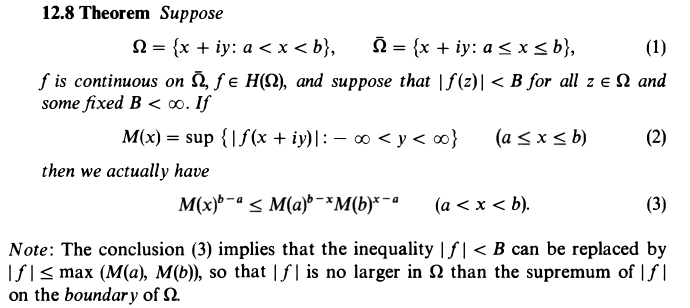
\includegraphics[width=\textwidth]{1-最大模原理-2025040417.png}
% \caption{}
\label{}
\end{figure}

\begin{figure}[H]
\centering
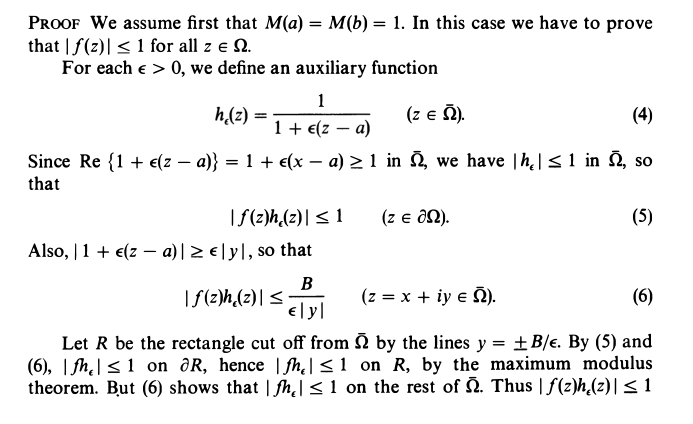
\includegraphics[width=\textwidth]{2-最大模原理-2025040417.png}
% \caption{}
\label{}
\end{figure}

\begin{figure}[H]
\centering
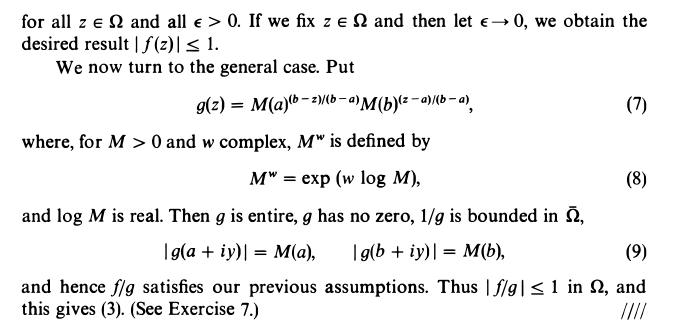
\includegraphics[width=\textwidth]{3-最大模原理-2025040417.png}
% \caption{}
\label{}
\end{figure}
